\documentclass[12pt, twoside]{article}
\usepackage[letterpaper, margin=1in, headsep=0.2in]{geometry}
\setlength{\headheight}{0.6in}
%\usepackage[english]{babel}
\usepackage[utf8]{inputenc}
\usepackage{microtype}
\usepackage{amsmath}
\usepackage{amssymb}
%\usepackage{amsfonts}
\usepackage{siunitx} %units in math. eg 20\milli\meter
\usepackage{yhmath} % for arcs, overparenth command
\usepackage{tikz} %graphics
\usetikzlibrary{quotes, angles}
\usepackage{graphicx} %consider setting \graphicspath{{images/}}
\usepackage{parskip} %no paragraph indent
\usepackage{enumitem}
\usepackage{multicol}
\usepackage{venndiagram}

\usepackage{fancyhdr}
\pagestyle{fancy}
\fancyhf{}
\renewcommand{\headrulewidth}{0pt} % disable the underline of the header
\raggedbottom
\hfuzz=2mm %suppresses overfull box warnings

\usepackage{hyperref}

\fancyhead[LE]{\thepage}
\fancyhead[RO]{\thepage \\ Name: \hspace{4cm} \,\\}
\fancyhead[LO]{BECA / Dr. Huson / Geometry\\*  Unit 8: Congruence transformations\\* 13 January 2023}

\begin{document}

\subsubsection*{8.9 Homework: Mixed review \hfill CCSS.HSG.CO.A.5}
\begin{enumerate}
  \item Given the situation in the diagram, answer each question. Circle True or False. %\vspace{1cm}
  \begin{flushright}
  \begin{tikzpicture}[scale=0.8]
    \draw [->, thick] (0,0)--(4,3);
    \draw [<->, thick] (-5,.5)--(5,-.5);
    \draw [->, thick] (0,0)--(-1.2,3);
    \draw [fill] (-1,2.5) circle [radius=0.05] node[left ]{$S$};
    \draw [fill] (2.66666,2) circle [radius=0.05] node[above left ]{$T$};
    \draw [fill] (0,0) circle [radius=0.05] node[below]{$P$};
    \draw [fill] (4,-0.4) circle [radius=0.05] node[above]{$U$};
    \draw [fill] (-4,0.4) circle [radius=0.05] node[above]{$R$};
  \end{tikzpicture}
  \end{flushright}
\begin{enumerate}
  \item True or False: $\angle SPU$ is an acute angle.
  \item True or False: $\overrightarrow{RP}$ and $\overrightarrow{PU}$ are opposite rays.
  \item True or False: $\angle RPS$ and $\angle SPU$ are a linear pair.
  \item True or False: $\angle SPT$ and $\angle TPR$ are adjacent.
\end{enumerate}

\item Construct an equilateral triangle having one side on $\overrightarrow{T}$ with each leg congruent to $\overline{AB}$.
[Leave all construction marks.]\\
  \vspace{3cm}
  \begin{center}
  \begin{tikzpicture}
    \draw [-, thick] (0,3)--(3,0);
    \draw [->, thick] (4,-3)--(11,-3);
    \draw [fill] (4,-3) circle [radius=0.05] node[above left]{$T$};
    \draw [fill] (0,3) circle [radius=0.05] node[above left]{$A$};
    %\node at (8.5,-0.4){$l$};
    \draw [fill] (3,0) circle [radius=0.05] node[below right]{$B$};
  \end{tikzpicture}
  \end{center}
  %\vspace{2cm}

\newpage
\item Given two parallel lines and a transversal, as shown. Apply the theorem, ``If a transversal intersects two parallel lines, then corresponding angles are congruent."
\begin{center}
\begin{tikzpicture}
\draw [<->, thick] (1,2)--(9,2);
\draw [<->, thick] (0,0)--(8,0);
\draw [<->, thick] (4,-1)--(5.5,3);
\node at (4.5,0.3) [left]{$5$};
\node at (4.5,0.3) [right]{$6$};
\node at (4.3,-0.3) [left]{$7$};
\node at (4.3,-0.3) [right]{$8$};
\node at (5.2,2) [above left]{$1$};
\node at (5.2,2) [above right]{$2$};
\node at (5,2) [below left]{$3$};
\node at (5,2) [below right]{$4$};
\end{tikzpicture}
\end{center}
\begin{enumerate}
\item State the angle corresponding with $\angle 1$. \bigskip
\item Given $m\angle 7 = 75^\circ$ and $m\angle 3 = 5x^\circ$. Find $x$. \bigskip
\item Given $m\angle 4 = 105^\circ$. Find $m\angle 6$. \bigskip
\item In a proof, what reason would justify $\angle 3 \cong \angle 6$? \rule{6cm}{0.15mm}
\end{enumerate}

\item Given two vertical angles, $m \angle 1 = 5x+13$, $m \angle 2 = 7x-11$. Find $m \angle 1$.\\
For full credit, check by comparing to $m\angle 2$.
  \begin{flushright}
  \begin{tikzpicture}[scale=.7]
    \draw [<->, thick] (0,-1.5)--(10,1.5);
    \draw [<->, thick] (2,3.5)--(7,-3.5);
    \node at (3,.4){1};
    \node at (6,-.6){2};
  \end{tikzpicture}
  \end{flushright}

\end{enumerate}

\newpage %BEGIN FIRST Page and remaining test questions
\setcounter{page}{1}
\subsubsection*{Trimester Final Exam}
You may use your notebook. No papers or loose notes.

\begin{enumerate}

\item Given the situation in the diagram, answer each question. Circle True or False. %\vspace{1cm}
  \begin{flushleft}
  \begin{tikzpicture}[scale=0.8]
    \draw [->, thick] (0,0)--(4,3);
    \draw [<->, thick] (-5,.5)--(5,-.5);
    \draw [->, thick] (0,0)--(-1.2,3);
    \draw [fill] (-1,2.5) circle [radius=0.05] node[left ]{$S$};
    \draw [fill] (2.66666,2) circle [radius=0.05] node[above left ]{$T$};
    \draw [fill] (0,0) circle [radius=0.05] node[below]{$P$};
    \draw [fill] (4,-0.4) circle [radius=0.05] node[above]{$U$};
    \draw [fill] (-4,0.4) circle [radius=0.05] node[above]{$R$};
  \end{tikzpicture}
\end{flushleft}
\begin{enumerate}
  \item True or False: $\angle SPU$ is an acute angle.
  \item True or False: $\overrightarrow{RP}$ and $\overrightarrow{PU}$ are opposite rays.
  \item True or False: $\angle RPS$ and $\angle SPU$ are a linear pair.
  \item True or False: $\angle SPT$ and $\angle TPR$ are adjacent.
\end{enumerate}

\item Given two parallel lines and a transversal, as shown. Apply the theorem, ``If a transversal intersects two parallel lines, then corresponding angles are congruent."
\begin{center}
\begin{tikzpicture}
  \draw [<->, thick] (1,2)--(9,2);
  \draw [<->, thick] (0,0)--(8,0);
  \draw [<->, thick] (4,-1)--(5.5,3);
  \node at (4.5,0.3) [left]{$5$};
  \node at (4.5,0.3) [right]{$6$};
  \node at (4.3,-0.3) [left]{$7$};
  \node at (4.3,-0.3) [right]{$8$};
  \node at (5.2,2) [above left]{$1$};
  \node at (5.2,2) [above right]{$2$};
  \node at (5,2) [below left]{$3$};
  \node at (5,2) [below right]{$4$};
\end{tikzpicture}
\end{center}
\begin{enumerate}
  \item State the angle corresponding with $\angle 1$. \bigskip
  \item Given $m\angle 7 = 75^\circ$ and $m\angle 3 = 5x^\circ$. Find $x$. \bigskip
  \item Given $m\angle 4 = 105^\circ$. Find $m\angle 6$. \bigskip
  \item In a proof, what reason would justify $\angle 3 \cong \angle 6$? \rule{6cm}{0.15mm}
\end{enumerate}

\newpage
\item Construct an equilateral triangle having one side on $\overrightarrow{T}$ with each leg congruent to $\overline{AB}$.
[Leave all construction marks.]\\
  \vspace{1cm}
  \begin{center}
  \begin{tikzpicture}
    \draw [-, thick] (0,3)--(3,0);
    \draw [->, thick] (4,-3)--(11,-3);
    \draw [fill] (4,-3) circle [radius=0.05] node[above left]{$T$};
    \draw [fill] (0,3) circle [radius=0.05] node[above left]{$A$};
    %\node at (8.5,-0.4){$l$};
    \draw [fill] (3,0) circle [radius=0.05] node[below right]{$B$};
  \end{tikzpicture}
  \end{center}
  \vspace{2cm}

\item Given two vertical angles, $m \angle 1 = 5x+13$, $m \angle 2 = 7x-11$. Find $m \angle 1$.\\
For full credit, check by comparing to $m\angle 2$.
  \begin{flushright}
  \begin{tikzpicture}[scale=.7]
    \draw [<->, thick] (0,-1.5)--(10,1.5);
    \draw [<->, thick] (2,3.5)--(7,-3.5);
    \node at (3,.4){1};
    \node at (6,-.6){2};
  \end{tikzpicture}
  \end{flushright}


\newpage %THE FOLLOWING PAGES are common to both versions

\item Given the square $EASY$ with $E(2, 1)$, $A(7, 1)$, $S(7, 6)$, and $Y(2, 6)$.
\begin{enumerate}
  \item Draw $EASY$ on the graph, labeling the vertices.
  \item Find the area of $EASY$. \vspace{2cm}
  \item Find the perimeter of $EASY$. \vspace{3cm}
\end{enumerate}
  \begin{tikzpicture}[scale=.635]
    \draw [help lines] (-3,-3) grid (8,8);
    \draw [thick, ->] (-3.2,0) -- (8.4,0) node [below right] {$x$};
    \draw [thick, ->] (0,-3.2)--(0,8.4) node [left] {$y$};
  \end{tikzpicture}

\item Given $m\angle R=45$, $m\angle U =55$, and $m\angle UST=100$. Find $m\angle RSU$.\\[1cm]
\begin{tikzpicture}
  %\draw [->, thick] (0,0)--(5,5);
  \draw [<-, thick] (8,0)--(0,0)--(3,3)--(4.5,0);
  \draw [fill] (0,0) circle [radius=0.05] node[below]{$R$};
  \draw [fill] (4.5,0) circle [radius=0.05] node[below]{$S$};
  \draw [fill] (3,3) circle [radius=0.05] node[right]{$U$};
  \draw [fill] (7,0) circle [radius=0.05] node[below]{$T$};
\end{tikzpicture}
\vspace{3cm}

\newpage
\item Construct a perpendicular bisector the given line segment $\overline{AB}$. Label the midpoint of $\overline{AB}$ as $M$.  [Leave all construction marks.]\\
\vspace{2cm}
\begin{center}
\begin{tikzpicture}
\draw [-, thick] (0,3)--(3,0);
\draw [fill] (0,3) circle [radius=0.05] node[above left]{$A$};
%\node at (8.5,-0.4){$l$};
\draw [fill] (3,0) circle [radius=0.05] node[below right]{$B$};
\end{tikzpicture}
\end{center}
\vspace{2cm}

\item Construct an angle bisector the given angle $A$.  [Leave all construction marks.]\\
\vspace{2cm}
\begin{center}
\begin{tikzpicture}
  \draw [<->, thick] (-2,5)--(0,0)--(7,0);
  \draw [fill] (0,0) circle [radius=0.05] node[below]{$A$};
  %\draw [fill] (7,0) circle [radius=0.05] node[below]{$N$};
\end{tikzpicture}
\end{center}

\newpage

\item On the graph below, draw $\overline{CD}$, with $C(-2,3)$ and $D(6,7)$, labeling the end points. Determine and state the coordinates of the midpoint $M$ of $\overline{CD}$ and mark and label it on the graph.\\
\begin{tikzpicture}[scale=.635]
  \draw [help lines] (-3,-3) grid (8,8);
  \draw [thick, ->] (-3.2,0) -- (8.4,0) node [below right] {$x$};
  \draw [thick, ->] (0,-3.2)--(0,8.4) node [left] {$y$};
\end{tikzpicture}
\vspace{2cm}

\item In a proof, each of the following statements are written. Write down the reason that would justify each step. \bigskip
\begin{enumerate}
  \item $PQ+RS= QR+RS$  \hspace{1.7cm} $\rule{5cm}{0.15mm}$ property  \bigskip
  \item $2(PQ + QR)=2PQ+2QR$  \hspace{0.6cm} $\rule{5cm}{0.15mm}$ property \bigskip
  \item $\overline{PQ} \cong \overline{PQ}$ \hspace{4cm} $\rule{5cm}{0.15mm}$ property
\end{enumerate}

\item Given a circle $O$ with radius $7$.
\begin{enumerate}
\item Find the circumference of $O$. \vspace{2cm}
\item Find the area of $O$.
\end{enumerate}

\newpage
\item Given two parallel lines and a transversal, as shown. $m\angle 2=7x+19$ and $m\angle 5=10x+8$. Find $m\angle 5$. Show the check for full credit.
\begin{flushleft}
\begin{tikzpicture}
\draw [<->, thick] (1,2)--(9,2);
\draw [<->, thick] (0,0)--(8,0);
\draw [<->, thick] (4,-1)--(5.5,3);
\node at (4.5,0.3) [left]{$5$};
%\node at (4.5,0.3) [right]{$6$};
%\node at (4.3,-0.3) [left]{$7$};
%\node at (4.3,-0.3) [right]{$8$};
%\node at (5.2,2) [above left]{$1$};
\node at (5.2,2) [above right]{$2$};
\node at (5,2) [below left]{$3$};
%\node at (5,2) [below right]{$4$};
\end{tikzpicture}
\end{flushleft}
\vspace{3cm}


\item Construct a perpendicular to $\overline{AB}$ through $C$.\\
%\hspace{1cm} Given the line  $l$ and point $P$.
\vspace{2cm}
\begin{center}
\begin{tikzpicture}
  \draw [<->, thick] (0,0)--(11,0)--(7,3)--cycle;
  \draw [fill] (0,0) circle [radius=0.05] node[left]{$A$};
  \draw [fill] (11,0) circle [radius=0.05] node[right]{$B$};
  \draw [fill] (7,3) circle [radius=0.05] node[above right]{$C$};
\end{tikzpicture}
\end{center}
%\vspace{4cm}

\newpage


\subsubsection*{Circle the appropriate equation and state the justification}
Use the postulates and theorems you have learned. You may abbreviate them as follows: ``def. of bisector," ``$\perp$ rays meet at $90^\circ$," ``complementary $\angle$s add to 90," ``linear pairs add to 180," ``vertical $\angle$s are $\cong$," ``corresponding $\angle$s of parallel lines are $\cong$."

\item Given corresponding angles of a transversal and two parallel lines, $\angle A$, $\angle B$.\\[0.5cm]
$\angle A \cong \angle B$ \hspace{1cm} $m \angle A + m \angle B=180^\circ$ \hspace{0.5cm} \rule{5cm}{0.15mm} \vspace{0.25cm}

\item $\angle RPS \cong \angle SPU$ \hspace{0.25cm} $m \angle RPS + m \angle SPU = 180^\circ$ \hspace{0.25cm} \rule{6cm}{0.15mm}  \vspace{0.25cm}
\begin{tikzpicture}[scale=0.7]
  \draw [<->, thick] (-5,.5)--(3,-.3);
  \draw [->, thick] (0,0)--(-1.2,3);
  \draw [fill] (-1,2.5) circle [radius=0.05] node[left ]{$S$};
  \draw [fill] (0,0) circle [radius=0.05] node[below]{$P$};
  \draw [fill] (2,-0.2) circle [radius=0.05] node[above]{$U$};
  \draw [fill] (-4,0.4) circle [radius=0.05] node[above]{$R$};
\end{tikzpicture}

\item Given $m \angle 1 = 4x+6$, $m \angle 2 = 6x-32$. Find $m \angle 1$.
\begin{tikzpicture}[scale=.4]
  \draw [<->, thick] (0,-1.5)--(10,1.5);
  \draw [<->, thick] (2,3.5)--(7,-3.5);
  \node at (3,.4){1};
  \node at (6,-.6){2};
\end{tikzpicture}\\[0.5cm]
$\angle 1 \cong \angle 2$ \hspace{1cm} $m\angle 1 + m\angle 2 =  180$ \hspace{0.5cm} \rule{6cm}{0.15mm}

\item Given $m\angle R=m\angle U =65$, and $m\angle UST=130$. Find $m\angle RSU$.
\begin{tikzpicture}[scale=0.6]
%\draw [->, thick] (0,0)--(5,5);
\draw [<-, thick] (7,0)--(1,0)--(3,3)--(4.5,0);
\draw [fill] (1,0) circle [radius=0.05] node[below]{$R$};
\draw [fill] (4.5,0) circle [radius=0.05] node[below]{$S$};
\draw [fill] (3,3) circle [radius=0.05] node[right]{$U$};
\draw [fill] (6,0) circle [radius=0.05] node[below]{$T$};
\end{tikzpicture}\\[0.5cm]
$\angle UST \cong \angle RSU$ \hspace{0.5cm} $m\angle UST + m\angle RSU =  180$ \hspace{0.5cm} \rule{6cm}{0.15mm} \vspace{0.5cm}

\item Given $\overrightarrow{BA} \perp \overrightarrow{BC}$, $m \angle ABD = 2x-5$, and $m \angle DBC = x-10$.
\begin{tikzpicture}[scale=0.7]
\draw [<->, thick] (0,3)--(0,0)--(5,0);
\draw [->, thick] (0,0)--(3.5, 2);
\draw [-, thin] (0, 0.4)--(0.4, 0.4)--(0.4, 0);
\draw [fill] (0,0) circle [radius=0.05] node[below]{$B$};
\draw [fill] (0,2) circle [radius=0.05] node[left]{$A$};
\draw [fill] (4,0) circle [radius=0.05] node[below]{$C$};
\draw [fill] (2.625, 1.5) circle [radius=0.05] node[below]{$D$};
\end{tikzpicture}\\[0.5cm]
$\angle ABD \cong \angle DBC$ \hspace{0.5cm} $m\angle ABD + m\angle DBC =  90$ \hspace{0.5cm} \rule{6cm}{0.15mm}


\newpage
\item Given $N(-8, -1)$, $Y(4, -1)$, and $C(4, 4)$.
\begin{enumerate}
  \item Plot and label the points on the graph, drawing $\overline{NC}$
  \item Draw the legs of the right triangle, $\overline{NY}$ and $\overline{YC}$, marking their lengths.
  \item Write down the distance formula for $NC$, substituting coordinate values.
  \item Find the value of $NC$.
\end{enumerate}
\begin{tikzpicture}[scale=.635]
  \draw [help lines] (-9,-5) grid (7,7);
  \draw [thick, ->] (-9.2,0) -- (7.4,0) node [below right] {$x$};
  \draw [thick, ->] (0,-5.2)--(0,7.4) node [left] {$y$};
\end{tikzpicture}
\vspace{3cm}

\item Given $\overline{ABC}$, $AC=15$, and the point $B$ partitions $\overline{AC}$ in a ratio of 1:2.\\[0.5cm] Find ${AB}$. \\[1.5cm]
  \begin{tikzpicture}
    \draw [-, thick] (1,0)--(7,0);
    \draw [fill] (1,0) circle [radius=0.05] node[below]{$A$};
    \draw [fill] (3.5,0) circle [radius=0.05] node[below]{$B$};
    \draw [fill] (7,0) circle [radius=0.05] node[below]{$C$};
  \end{tikzpicture} \vspace{3cm}

\newpage

\item Construct the midpoint $M$ of $\overline{AC}$ by using the perpendicular bisector construction. Draw $\overline{BM}$, a \emph{median} of $\triangle ABC$.\\
Spicy: Construct the other two medians, and hence, their intersection, the centroid.
\vspace{5cm}
\begin{center}
\begin{tikzpicture}[scale=1.2]
  \draw [<->, thick] (0,0)--(6.5,0)--(6,4)--cycle;
  \draw [fill] (0,0) circle [radius=0.05] node[left]{$A$};
  \draw [fill] (6.5,0) circle [radius=0.05] node[right]{$B$};
  \draw [fill] (6,4) circle [radius=0.05] node[above right]{$C$};
\end{tikzpicture}
\end{center} \vspace{1.5cm}

\newpage

\item Given $\overrightarrow{BA} \perp \overrightarrow{BC}$, $m \angle ABD = 5x$, and $m \angle DBC = 2x-1$. Find $m \angle DBC$. \\[0.5cm]
For full credit, show the check using both angle measures.
\begin{flushleft}
\begin{tikzpicture}[scale=1.3]
  \draw [<->, thick] (0,3)--(0,0)--(5,0);
  \draw [->, thick] (0,0)--(3.5, 2);
  \draw [-, thin] (0, 0.4)--(0.4, 0.4)--(0.4, 0);
  %\node at (3,.4){1};
  %\node at (6,-.6){2};
  \draw [fill] (0,0) circle [radius=0.05] node[below]{$B$};
  \draw [fill] (0,2) circle [radius=0.05] node[left]{$A$};
  \draw [fill] (4,0) circle [radius=0.05] node[below]{$C$};
  \draw [fill] (2.625, 1.5) circle [radius=0.05] node[below]{$D$};
\end{tikzpicture}
\end{flushleft}
\vspace{5cm}


\item Given $\overleftrightarrow{QS}$ as shown on the number line, with $Q$ having the coordinate 1.8 and $S$ the coordinate 4.7. \\[6pt] % Midpoint
\begin{tikzpicture}
  \draw [<->] (-4.5,0)--(6.5,0);
  \foreach \x in {-4,...,6} %2 leading for diff!=1
    \draw[shift={(\x,0)},color=black] (0pt,-3pt) -- (0pt,3pt) node[below=5pt]  {$\x$};
    \draw [fill] (1.8,0) circle [radius=0.05] node[above] {$Q$};
    \draw [fill] (4.7,0) circle [radius=0.05] node[above] {$S$};
\end{tikzpicture} \bigskip
\begin{enumerate}
  \item Find the value of the coordinate of the point $R$, the midpoint of $\overline{QS}$. \vspace{3cm}
  \item The point $P$ is collinear with $\overleftrightarrow{QS}$ such that $Q$ is the midpoint of $\overleftrightarrow{PS}$. Mark $P$ on the line and state the value of its coordinate.
\end{enumerate} %\vspace{4cm}

\newpage

\item Given $M(-2,4)$ and $N(6,-2)$, find the length of $\overline{MN}$.
  \vspace{6cm}

\item Construct a duplicate of the given angle $A$.  [Leave all construction marks.]\\[3cm]
  %\vspace{2cm}
  %\begin{center}
  \begin{tikzpicture}
    \draw [<->, thick] (3,5)--(0,0)--(6,0);
    \draw [fill] (0,0) circle [radius=0.05] node[below]{$A$};
    %\draw [fill] (7,0) circle [radius=0.05] node[below]{$N$};
  \end{tikzpicture}
  %\end{center}

\newpage

\item Prove the quadrilateral $BECA$ with $B(1, 3)$, $E(3, 2)$, $C(5,6)$, and $A(3, 7)$ is a rectangle, using the theorem ``If a quadrilateral's diagonals are congruent, then it is a rectangle."
\begin{enumerate}
\item Draw $BECA$, labeling the vertices, and draw the diagonals, $\overline{BC}$ and $\overline{EA}$.
\item Find the length $EA$, showing the subtraction of the $y$ values, and $BC$, using the distance formula.
\item State the theorem above to complete the proof.
\end{enumerate}
\begin{tikzpicture}[scale=.635]
\draw [help lines] (-2,-2) grid (8,8);
\draw [thick, ->] (-2.2,0) -- (8.4,0) node [below right] {$x$};
\draw [thick, ->] (0,-2.2)--(0,8.4) node [left] {$y$};
\end{tikzpicture}
\vspace{2cm}

\item Given the circle $C$ with circumference $6\pi$.
\begin{enumerate}
\item Write down the formula for the circumference of a circle and solve for the radius yielding a circumference of $6\pi$. \vspace{1cm}
\item Find the area of the circle.
\end{enumerate}
\begin{tikzpicture}[scale=.635]
\draw [help lines] (-4,-4) grid (4,4);
%\draw [thick, ->] (-2.2,0) -- (10.4,0) node [below right] {$x$};
%\draw [thick, ->] (0,-2.2)--(0,10.4) node [left] {$y$};
\draw (0,0) circle [radius=3] node[below]{$C$};
\draw [fill] (0,0) circle [radius=0.05];
\end{tikzpicture}

\newpage
\item On the graph, draw polygon ABCDEF with vertices A(0, 0), B(0, 7), C(5, 7), D(5, 4), E(8, 4), and F(8, 0). Find the perimeter and the area of the polygon.\\[1cm]
\begin{tikzpicture}[scale=.635]
\draw [help lines] (-2,-2) grid (10,10);
\draw [thick, ->] (-2.2,0) -- (10.4,0) node [below right] {$x$};
\draw [thick, ->] (0,-2.2)--(0,10.4) node [left] {$y$};
\end{tikzpicture}
\vspace{2cm}

\item In the circle below, $\overline{AB}$ is a chord. Using a compass and straightedge, construct a perpendicular bisector of $\overline{AB}$, and hence, a diameter of the circle. \\
(Leave all construction marks.)
\vspace{2cm}
\begin{center}
\begin{tikzpicture}[scale=.5]
  %\draw [help lines] (-4,-4) grid (4,4);
  \draw [thick, -] (-5,0) node[left]{$A$} -- (0,5) node[above]{$B$};
  %\draw [thick, ->] (0,-2.2)--(0,10.4) node [left] {$y$};
  \draw (0,0) circle [radius=5]; %node[below]{$C$};
  %\draw [fill] (0,0) circle [radius=0.05];
\end{tikzpicture}
\end{center}

\newpage
\item Construct the angle bisectors of the angles of the triangle and their intersection, the incenter.\\
%\hspace{1cm} Given the line  $l$ and point $P$.
\vspace{3cm}
\begin{center}
\begin{tikzpicture}[scale=1.2]
  \draw [<->, thick] (0,0)--(9,0)--(7,11)--cycle;
  %\draw [fill] (2,3) circle [radius=0.05] node[right]{$P$};
  %\node at (8.5,-0.4){$l$};
  %\draw [fill] (6,0) circle [radius=0.05] node[below]{$Q$};
\end{tikzpicture}
\end{center}

\newpage
\item Given the quadrilateral $RSTU$ with $R(-8,-1)$, $S(2,-1)$, $T(10,5)$, and $U(0,5)$.
\begin{enumerate}
\item Plot and label $RSTU$ on the grid.
\item Using the distance formula or otherwise, calculate $RS$, $ST$, $TU$, and $RU$.
\item Definition: If a quadrilateral has four congruent sides, then it is a rhombus.\\[0.5cm]
Prove that $RSTU$ is a rhombus.
\end{enumerate}

\begin{center} %4 quadrant regents grid w T-Chart
\begin{tikzpicture}[scale=.635]
\draw [help lines] (-10,-5) grid (10,10);
\draw [thick, ->] (-10.2,0) -- (10.4,0) node [below right] {$x$};
\draw [thick, ->] (0,-5.2)--(0,10.4) node [left] {$y$};
\end{tikzpicture}
\end{center}

\newpage
\item A duplicate of $\angle ABC$ is constructed with $A$ as the vertex. The new leg of $\angle A$ is parallel to $\overleftrightarrow{BC}$, and labeled $l$.
\vspace{2cm}
  \begin{center}
  \begin{tikzpicture}[scale=1.4]
    \draw [<->, thick] (-1,0)--(0,0)--(4,0);
    \draw [<->, thick] (-1,-1)--(5,5);
    \draw [->, thick] (2.5,2.5)--(5, 2.5) node[below right]{$l$};
    \draw [fill] (2.5,2.5) circle [radius=0.05] node[above left]{$A$};
    \draw [fill] (0,0) circle [radius=0.05] node[above left]{$B$};
    \draw [fill] (3,0) circle [radius=0.05] node[above left]{$C$};
    %\draw [fill] (7,0) circle [radius=0.05] node[above right]{$C$};
  \end{tikzpicture}
  \end{center}
  \vspace{1cm}
  \begin{enumerate}
    \item Are $\angle A$ and $\angle B$ complementary, supplementary, or congruent? Justify your answer. \vspace{3cm}
    \item Would $\angle A$ and $\angle B$ be considered corresponding, alternate interior angles, or same-side exterior angles?
  \end{enumerate}


\end{enumerate}
\end{document}

